%% abtex2-modelo-trabalho-academico.tex, v-1.7.1 laurocesar
%% Copyright 2012-2013 by abnTeX2 group at http://abntex2.googlecode.com/ 
%%
%% This work may be distributed and/or modified under the
%% conditions of the LaTeX Project Public License, either version 1.3
%% of this license or (at your option) any later version.
%% The latest version of this license is in
%%   http://www.latex-project.org/lppl.txt
%% and version 1.3 or later is part of all distributions of LaTeX
%% version 2005/12/01 or later.
%%
%% This work has the LPPL maintenance status `maintained'.
%% 
%% The Current Maintainer of this work is the abnTeX2 team, led
%% by Lauro César Araujo. Further information are available on 
%% http://abntex2.googlecode.com/
%%
%% This work consists of the files abntex2-modelo-trabalho-academico.tex,
%% abntex2-modelo-include-comandos and abntex2-modelo-references.bib
%%

% ------------------------------------------------------------------------
% ------------------------------------------------------------------------
% abnTeX2: Modelo de Trabalho Academico (tese de doutorado, dissertacao de
% mestrado e trabalhos monograficos em geral) em conformidade com 
% ABNT NBR 14724:2011: Informacao e documentacao - Trabalhos academicos -
% Apresentacao
% ------------------------------------------------------------------------
% ------------------------------------------------------------------------


%%%%%%%%%%%%%%%%%%
%
% As alterações realizadas no leiaute original do abntex2 disponibilizado 
% no sharelatex adaptaram o leiaute do abntex2 aos requisitos mínimos
% para escrita de dissertações e teses customizadas para o 
% centro de informática da ufpe.
%
% Bruno Maciel <bifm@cin.ufpe.com> 20/10/2016
% Daniel Severo Estrázulas <dse@cin.ufpe.br> 19/10/2020
% Alterações realizadas para o template da biblioteca atualizado disponibilizado no site Versão 07.10.2020 (1.3) revisado pelas bibliotecárias do setor bibccen.pt@ufpe.br
%%%%%%%%%%%%%%%%%%%%%%%%%%%%%%%%%%%%%%%%%%%%%%%%%%%%%%%%%%%%%%%

\documentclass[
	% -- opções da classe memoir --
	12pt,				% tamanho da fonte
	openright,			% capítulos começam em pág ímpar (insere página vazia caso preciso)
	oneside,			% para impressão em verso e anverso. Oposto a oneside
	a4paper,			% tamanho do papel. 
	% -- opções da classe abntex2 --
	chapter=TITLE,		% títulos de capítulos convertidos em letras maiúsculas
	section=TITLE,		% títulos de seções convertidos em letras maiúsculas
	%subsection=TITLE,	% títulos de subseções convertidos em letras maiúsculas
	%subsubsection=TITLE,% títulos de subsubseções convertidos em letras maiúsculas
	% -- opções do pacote babel --
	english,			% idioma adicional para hifenização
	french,				% idioma adicional para hifenização
	spanish,			% idioma adicional para hifenização
	brazil,				% o último idioma é o principal do documento
	english,
	brazil,
	]{abntex2/abntex2}
	\renewcommand{\baselinestretch}{1.5} %para customizar o espaço entre as linhas do texto
% --
% SETTINGS
\addto\captionsenglish{\renewcommand{\listfigurename}{List of Figures}}
\usepackage{abntex2/abntex2-cin-ufpe}
\usepackage[english]{babel}

% \usepackage[noframe]{showframe}
% \usepackage{showframe}

%\overfullrule=4mm %para identificar onde existem os alertas de linhas grandes mal formatada pelo LaTex, basta comentar para não aparecer a barra lateral preta na linha em questão.

\renewcommand*\arraystretch{1.2} %para customizar o espaço entre as linhas das tabelas


\usepackage{pdfpages} %para incluir pdf como páginas


% ---
% PACOTES
% ---
\usepackage{float}
\usepackage{cmap}				% Mapear caracteres especiais no PDF
\usepackage{lmodern}			% Usa a fonte Latin Modern			
\usepackage[T1]{fontenc}		% Selecao de codigos de fonte.
\usepackage[utf8]{inputenc}		% Codificacao do documento (conversão automática dos acentos)
\usepackage{lastpage}			% Usado pela Ficha catalográfica
\usepackage{indentfirst}		% Indenta o primeiro parágrafo de cada seção.
%\usepackage{color}				% Controle das cores
\usepackage{graphicx}			% Inclusão de gráficos
\usepackage{lipsum}				% para geração de dummy text
\usepackage[versalete,alf,abnt-and-type=e,abnt-etal-list=0,abnt-etal-cite=3]{abntex2/abntex2cite} 
\usepackage{multirow}
\usepackage[section]{placeins}



% -----------------------------------------------------------
% lista de abreviaturas e siglas
% início
% -----------------------------------------------------------
% \usepackage[noredefwarn,acronym]{glossaries} %GLOSSÁRIO
\usepackage[acronym,nonumberlist,nogroupskip,noredefwarn]{glossaries}
% \usepackage{glossary-superragged}

\newcolumntype{L}[1]{>{\raggedright\let\newline\\\arraybackslash\hspace{0pt}}m{#1}}
\newcolumntype{C}[1]{>{\centering\let\newline\\\arraybackslash\hspace{0pt}}m{#1}}
\newcolumntype{R}[1]{>{\raggedleft\let\newline\\\arraybackslash\hspace{0pt}}m{#1}}

\newglossarystyle{modsuper}{%
  \glossarystyle{super}%
  \renewcommand{\glsgroupskip}{}
  
  % put the glossary in a longtable environment:
 \renewenvironment{theglossary}%
  {
    \begin{longtable}
        {L{0.2\textwidth}L{0.8\textwidth}}}%
    {\end{longtable}
  }%
}

% -----------------------------------------------------------
% lista de abreviaturas e siglas
% fim
% -----------------------------------------------------------


\usepackage{lscape} 
\usepackage{rotating} %rotates the figures, page
\usepackage{tikz}
\usepackage[section]{placeins}
\usepackage{setspace} 



% ----------------------------------------------------------
% PERSONALIZAÇÃO DE CORES
% ----------------------------------------------------------
\definecolor{blue}{RGB}{41,5,195}
\definecolor{gray}{rgb}{.4,.4,.4}
\definecolor{gray}{rgb}{.4,.4,.4}
\definecolor{pblue}{rgb}{0.13,0.13,1}
\definecolor{pgreen}{rgb}{0,0.5,0}
\definecolor{pred}{rgb}{0.9,0,0}
\definecolor{pgrey}{rgb}{0.46,0.45,0.48}
\definecolor{lightgray}{rgb}{0.95, 0.95, 0.96}
\definecolor{whitesmoke}{rgb}{0.96, 0.96, 0.96}
\definecolor{javared}{rgb}{0.6,0,0} % for strings
\definecolor{javagreen}{rgb}{0.25,0.5,0.35} % comments
\definecolor{javapurple}{rgb}{0.5,0,0.35} % keywords
\definecolor{javadocblue}{rgb}{0.25,0.35,0.75} % javadoc
\definecolor{meucinza}{rgb}{0.5, 0.5, 0.5}
%\definecolor{lightgray}{gray}{0.9}


% ----------------------------------------------------------
% PERSONALIZAÇÃO DO USUÁRIO
% ----------------------------------------------------------

% ----------------------------------------------------------
% DADOS DO TRABALHO - CAPA e FOLHA DE ROSTO
% Configure os dados do trabalho aqui
% ----------------------------------------------------------
\titulo{\textbf{Isolating Feature Impacts in Educational Data Mining: Novel Metrics and Insights from Accumulated Local Effects}}
\autor{Rogério Luiz Cardoso Silva Filho}
\local{Recife}
\data{\Year}
\areaconcentracao{\textbf{Área de Concentração}: Inteligência Artificial}
\orientador{\textbf{Orientador (a)}: Paulo Jorge Leitão Adeodato}
\coorientador{\textbf{Coorientador (a)}: Kellyton dos Santos Brito}

\instituicao{UNIVERSIDADE FEDERAL DE PERNAMBUCO \\ CENTRO DE INFORMÁTICA \\PROGRAMA DE PÓS-GRADUAÇÃO EM CIÊNCIAS DA COMPUTAÇÃO}
\departamento{Centro de Informática}
\programa{Pós-graduação em Ciências da Computação}
\emailprograma{rlcsf@cin.ufpe.br}
\siteprograma{http://cin.ufpe.br/\textasciitilde posgraduacao}

\tipotrabalho{phdthesis}
% O preambulo deve conter o tipo do trabalho, o objetivo, 
% o nome da instituição e a área de concentração 
%\preambulo{Trabalho apresentado ao Programa de Pós-graduação em Ciência da Computação do Centro de Informática da Universidade Federal de Pernambuco, como requisito parcial para obtenção do grau de Doutor em Ciência da Computação.}

%\preambuloatadefesa{Dissertação apresentada ao Programa de Pós-Graduação Profissional em Ciência da Computação da Universidade Federal de Pernambuco, como requisito parcial para a obtenção do título de Doutor em 04 de setembro de 2020.}

\preambulo{Trabalho apresentado ao Programa de Pós-graduação em Ciência da Computação do Centro de Informática da Universidade Federal de Pernambuco, como requisito parcial para obtenção do grau de Doutor em Ciências da Computação}

\preambuloatadefesa{Texto texto texto texto texto texto texto texto texto texto texto texto texto texto texto texto texto texto texto texto texto texto texto texto texto texto texto texto texto texto texto texto.}




\input{userlists}






% ----------------------------------------------------------
% COMPILA O ÍNDICE
% ----------------------------------------------------------
\makeindex
% ---


% ----------------------------------------------------------
% LISTA E ABREVIATURAS E SIGLAS
% ----------------------------------------------------------
%lista de siglas
\newacronym{XAI}{XAI}{eXplainabe Artificial Intelligence}
\newacronym{ML}{ML}{Machine Learning}
\newacronym{EDM}{EDM}{Educational Data Mining}


\makenoidxglossaries
\renewcommand*{\glsseeformat}[3][\seename]{\textit{#1}  
\glsseelist{#2}}

\renewcommand*{\glspostdescription}{} % remove trailing dot
\renewcommand{\glsnamefont}[1]{\textbf{#1}}

\renewcommand{\familydefault}{\sfdefault}

% ----------------------------------------------------------
% GLOSSÁRIO
% ----------------------------------------------------------

\newglossaryentry{naive-bayes}
{
  name=\textit{Na{\"i}ve Bayes},
  description={},
  plural=\textit{Na{\"i}ve Bayes}
}

\newglossaryentry{hoeffding-tree}
{
  name=\textit{Hoeffding Tree},
  description={},
  plural=\textit{Hoeffding Trees}
}















\usepackage{pdfpages}
\usepackage{inconsolata}
\usepackage{listings}

\definecolor{cinza}{HTML}{FCF8F8}

% define formato e estilo dos elementos do tipo Codigo Fonte
\lstset{language=PHP,
basicstyle=\ttfamily\scriptsize,
%basicstyle=\ttfamily,
keywordstyle=\color{javapurple}\bfseries,
stringstyle=\color{pblue},
commentstyle=\color{javagreen},
morecomment=[s][\color{javadocblue}]{/**}{*/},
morecomment=[s][\color{gray}]{@}{\ },
numbers=left,
numberstyle=\tiny\color{black},
backgroundcolor=\color{cinza},
stepnumber=2,
numbersep=8pt,
xleftmargin=14pt,
tabsize=4,
showspaces=false,
showstringspaces=false,
breaklines=true,}

%%%%%%%%%%%%%%%%%%%%%%%%%%%%%%%%%%



\usepackage{adjustbox} % ajustar tabela ao tamanho da pagina
\usepackage{algpseudocode}
\usepackage{algorithm}
\usepackage{amsfonts}
\usepackage{amssymb}



% ----------------------------------------------------------
% INÍCIO DO DOCUMENTO
% ----------------------------------------------------------
\begin{document}

\frenchspacing % Retira espaço extra obsoleto entre as frases.

\imprimircapa
\imprimirfolhaderosto*~
%%a ficha deve ser passada pelo setor da biblioteca e sobrescrito no formato pdf

\includepdf[pages=-]{others/ficha.pdf}

%\newpage
%\input{others/ata_defesa}
%%a folha de aprovação deve ser um pdf que a secretaria encaminha sem assinaturas
%basta fazer upload na basta others e sobrescrever

\includepdf[pages=-]{others/folha_aprovacao_original}

% ----------------------------------------------------------
% DEDICATÓRIA
% ----------------------------------------------------------
\begin{dedicatoria}
   \vspace*{\fill}
%   \centering
  % \noindent
   %\textit{\lipsum[2]} 
   Dedico este trabalho aos meus pais, Rogério e Madalena, que excederam todos os seus limites para me dar a melhor educação, a minha amada esposa Alice, e ao meu querido filho Antônio, por todo amor e complacência.
   %\vspace*{\fill}
\end{dedicatoria}
% ---

%% ----------------------------------------------------------
% AGRADECIMENTOS
% ----------------------------------------------------------
\begin{agradecimentos}




\end{agradecimentos}


% ----------------------------------------------------------
% EPÍGRAFE

%Epígrafe: Elemento opcional e sem título em que o (a) autor (a) apresenta uma citação relacionada ao assunto tratado no trabalho. Deve ser elaborada conforme a ABNT-NBR 10520 (Citações). As citações de até três linhas devem estar entre aspas duplas e as citações com mais de três linhas devem ser destacadas com recuo de 4 cm da margem esquerda, com letra menor que a do texto e sem as aspas. A fonte da citação deve aparecer na lista de referências.
% ---------------------------------------------------------
\vspace*{10cm}
\begin{citacao}
\end{citacao}

    \vspace*{5cm}
	
		''Should philosophy guide experiments, or should experiments guide philosophy?'' (Liu Cixin) 
	
\newpage

% resumo em português
\begin{resumo}[Resumo] 
Esta tese apresenta um estudo na interseção entre Aprendizado de Máquina (ML) e educação, enfatizando a aplicação de técnicas de Inteligência Artificial Explicável (IAE) em Mineração de Dados Educacionais (MDE). Central para esta pesquisa é o desafio de fornecer explicações globais post-hoc para modelos de ML, especialmente quando a independência dos dados não pode ser assumida, uma questão comum, porém pouco explorada, em MDE. Ignorar interdependências de dados pode enviesar explicações, inflar variáveis irrelevantes ou atribuir desproporcionalmente significância a certos preditores. Para resolver esses desafios, a tese baseia-se em um método recente para a visualização do impacto das variáveis em modelos supervisionados, conhecido em inglês como Accumulated Local Effects (ALE), que se refere à distribuição acumulada de efeitos locais. A propriedade pseudo-ortogonal de ALE permite isolar os efeitos de variáveis individuais, distinguindo-a de métodos amplamente usados em MDE, como os gráficos de dependência parcial e explicações baseadas  em valores de Shapley. Para demonstrar as propriedades de ALE quando comparados com métodos tradicionais, este trabalho introduz uma nova metodologia para avaliação da capacidade de técnicas de IAE em aproximar o real comportamento de variáveis  em diversos contextos de dependência entre dados. Além disso, este trabalho propõe novas métricas baseadas em ALE para a medição do impacto de variáveis em modelos supervisionados. Essas métricas agnósticas a modelos são uma melhoria em relação às técnicas tradicionais, fornecendo percepções mais claras e precisas de como as variáveis afetam os resultados do modelo, incluindo tanto a extensão quanto a direção de seus impactos. A eficácia dessas métricas é demonstrada em conjuntos de dados sintéticos e reais, provando sua efetividade em isolar os efeitos de  variáveis relevantes para as predições dos modelos quando comparada com métricas existentes. Além disso, um estudo empírico utilizando os dados das escolas secundárias brasileiras não apenas ratifica a utilidade das novas métricas em cenários do mundo real, mas também estende as contribuições desta tese ao identificar e oferecer novas perspectivas sobre os determinantes do sucesso escolar brasileiro ao longo de uma década.

% \noindent %- o resumo deve ter apenas 1 parágrafo e sem recuo de texto na primeira linha, essa tag remove o recuo. Não pode haver quebra de linha.

 \vspace{\onelineskip}
    
 \noindent
 \textbf{Palavras-chaves}: IA explicável. Aprendizagem de máquina interpretável.  Explicadores globais. Mineração de dados educacionais. Importância de variáveis. ALE.
\end{resumo}

%resumo em inglês
\begin{resumo}[Abstract]
\begin{otherlanguage*}{english}

 %\noindent
This thesis presents a study at the intersection of Machine Learning (ML) and education, emphasizing the application of eXplainable Artificial Intelligence (XAI) techniques in Educational Data Mining (EDM). Central to this research is the challenge of providing post-hoc global explanations for ML models, especially when data independence cannot be assumed, a common yet underexplored issue in EDM. Overlooking data interdependencies can bias explanations, inflate irrelevant variables, or disproportionately attribute significance to certain predictors. To address these challenges, this work builds on Accumulated Local Effects (ALE), a recent method for post-hoc global explanation that visualizes the impact of features. ALE's pseudo-orthogonality property allows for isolating individual variable effects, distinguishing it from widely used methods in EDM, such as Partial Dependence (PD) Plots and SHapley Additive Explanations (SHAP). To showcase ALE's properties, this work introduces a new evaluation methodology to rigorously assess ALE's ability against established methods in approximating the true behavior of features across various data dependency contexts. Furthermore, this work proposes new metrics based on ALE, aimed at measuring feature impact sizes. These model-agnostic metrics are an improvement over traditional explanation scores, as they provide clearer and more accurate insights into how features affect model outcomes, including the extent and direction of their impacts. The efficacy of these metrics is demonstrated through comprehensive validation on both synthetic and real datasets, proving their effectiveness in isolating key variable effects compared to existing scores. Furthermore, the application of these metrics in an empirical study within Brazilian secondary schools not only underscores their practicality in real-world scenarios but also extends the contributions of this thesis by offering new perspectives on the determinants of educational outcomes in Brazilian secondary schools over a decade.

\vspace{\onelineskip} 

\noindent 
\textbf{Keywords}: Explaineble AI. Interpretable ML.  Global explainers. EDM. Feature importance. ALE.
\end{otherlanguage*}
\end{resumo}



% ----------------------------------------------------------
% LISTA DE FIGURAS
% ----------------------------------------------------------
\pdfbookmark[0]{\listfigurename}{lof}
\listoffigures*
\cleardoublepage



% ---
% LISTA DE CÓDIGOS FONTES
% ---

%\pdfbookmark[0]{\lstlistingname}{lol} % caso não tenha quadros, comente esta linha 
%\counterwithout{lstlisting}{chapter}



% Altera o nome padrão do rótulo usado no comando \autoref{}
%\renewcommand{\lstlistingname}{Código Fonte}

% Altera o rótulo a ser usando no elemento pré-textual "Lista de código"
\renewcommand{\lstlistlistingname}{Lista de códigos}

% Configura a ``Lista de Códigos'' conforme as regras da ABNT (para abnTeX2)
\begingroup\makeatletter
\let\newcounter\@gobble\let\setcounter\@gobbletwo
  \globaldefs\@ne \let\c@loldepth\@ne
  \newlistof{listings}{lol}{\lstlistlistingname}
  \newlistentry{lstlisting}{lol}{0}
\endgroup

\renewcommand{\cftlstlistingaftersnum}{\hfill--\hfil}

\let\oldlstlistoflistings\lstlistoflistings
{
\let\oldnumberline\numberline
\newcommand{\algnumberline}[1]{Código Fonte~#1~\enspace--~\enspace}
\renewcommand{\numberline}{\algnumberline}

\begin{KeepFromToc}
%\lstlistoflistings
\end{KeepFromToc}
}
\cleardoublepage

% ---
% LISTA DE QUADROS
% ---
%\pdfbookmark[0]{\listofquadrosname}{loq} % caso não tenha quadros, comente esta linha 
%\listofquadros* % caso não tenha quadros, comente esta linha 
\cleardoublepage



% ----------------------------------------------------------
% LISTA DE TABELAS
% ----------------------------------------------------------

\pdfbookmark[0]{\listtablename}{lot}
\listoftables*
\cleardoublepage


        
  
% ----------------------------------------------------------
% LISTA E ABREVIATURAS E SIGLAS
% ----------------------------------------------------------
% \printglossary[type=\acronymtype,title={\listadesiglasname},nonumberlist]
% \printglossaries
% compile uma vez com o comando \printglossaries e depois compile novamente com o comando \printglossaries comentado para as páginas glossário e siglas serem ocultadas.

% ----------------------------------------------------------
% LISTA E ABREVIATURAS E SIGLAS
% ----------------------------------------------------------
% \setglossarystyle{modsuper}
\printnoidxglossary[style=modsuper,type=\acronymtype,title={\listadesiglasname},nonumberlist]
% \printglossary[style=super, type=\acronymtype]
\cleardoublepage



% ----------------------------------------------------------
% LISTA DE SIMBOLOS
% ----------------------------------------------------------
%


% ---

% ---
% inserir lista de símbolos
% ---
\begin{simbolos}
  \item[$ \gamma $] Letra grega Gama
  %\item[$ \Lambda $] Lambda
  %\item[$ \zeta $] Letra grega minúscula zeta
  \item[$ \in $] Pertence
%  \item[$ \infty$] Infinito
%  \item[$ \ge$] Maior ou Igual
  \item[$ \delta$] Delta
  \item[$ \theta$] Teta
  \item[$ \sigma$] Sigma
  \item[$ \mu$] Mi
  
\end{simbolos}
% ---




% ----------------------------------------------------------
%


% ---

% ---
% inserir lista de símbolos
% ---
\begin{simbolos}
  \item[$ \gamma $] Letra grega Gama
  %\item[$ \Lambda $] Lambda
  %\item[$ \zeta $] Letra grega minúscula zeta
  \item[$ \in $] Pertence
%  \item[$ \infty$] Infinito
%  \item[$ \ge$] Maior ou Igual
  \item[$ \delta$] Delta
  \item[$ \theta$] Teta
  \item[$ \sigma$] Sigma
  \item[$ \mu$] Mi
  
\end{simbolos}
% ---






% ----------------------------------------------------------
% SUMÁRIO
% ----------------------------------------------------------
\renewcommand{\contentsname}{Table of Contents}
\pdfbookmark[0]{\contentsname}{toc}
\tableofcontents*
% \begingroup\intoctrue
% \tableofcontents*
% \endgroup
\cleardoublepage

% \setcounter{page}{13}
\setcounter{tocdepth}{2}
\setcounter{table}{0}




% ----------------------------------------------------------
% ELEMENTOS TEXTUAIS
% ----------------------------------------------------------
\textual

\section{Summary}

This chapter illustrated the significance of the proposed metrics in a real-world application: Identify and track the relevance of features in secondary educational outcomes in the Brazilian public educational system. The application was defined as a repeated cross-sectional analysis, which required a definition of a new process since, to our knowledge,  there are no other examples of this trend analysis using supervised learning. 

The findings of this study may also provide valuable insights for researchers interested in Brazilian secondary education. While it is well-established in the literature that factors such as \textit{income}, \textit{age}, \textit{race}, and \textit{parent's education} have a strong impact on educational achievement, it is still an open question as to how these factors evolve and influence achievement over the period of study. Moreover, student computers at school, which presents mixed findings regarding its effects in the literature, have been highlighted in this paper as one of the most effective policies regarding variables related to schools. Additionally, the knowledge extraction process leverages hypotheses that have either only been discussed qualitatively or not at all. For example, the study has suggested that improving \textit{Faculty education}, \textit{Faculty appropriate training} (especially for language teachers), and addressing Faculty workload could be important for improving secondary school achievement. Nevertheless, this investigation is not able to provide  causal conclusions, and further research by domain experts is needed to confirm the findings. 

\bookmarksetup{startatroot}% 


% ----------------------------------------------------------
% ELEMENTOS PÓS-TEXTUAIS
% ----------------------------------------------------------
\postextual


% ----------------------------------------------------------
% Referências bibliográficas
% ----------------------------------------------------------
\bibliographystyle{abntexalfenglish} %caso seja em inglês, retire o comentário desta linha

% \renewcommand{\bibname}{REFER\^ENCIAS}
%\renewcommand{\bibname}{Bibliography}
% \addbibresource{sample.bib}
\bibliography{references}


% ----------------------------------------------------------
% Apêndices
% ----------------------------------------------------------


% ----------------------
% força para que não exiba subtítulos em apêndices no sumário
% -----------------------

\begin{apendicesenv}
\addtocontents{toc}{\protect\setcounter{tocdepth}{1}}
\makeatletter
\addtocontents{toc}{%
  \begingroup
  \let\protect\l@chapter\protect\l@section
  \let\protect\l@section\protect\l@subsection
}
\makeatother

% Imprime uma página indicando o início dos apêndices
% \partapendices

%%coloca o identificador do anexo/apendice somente na primeira página
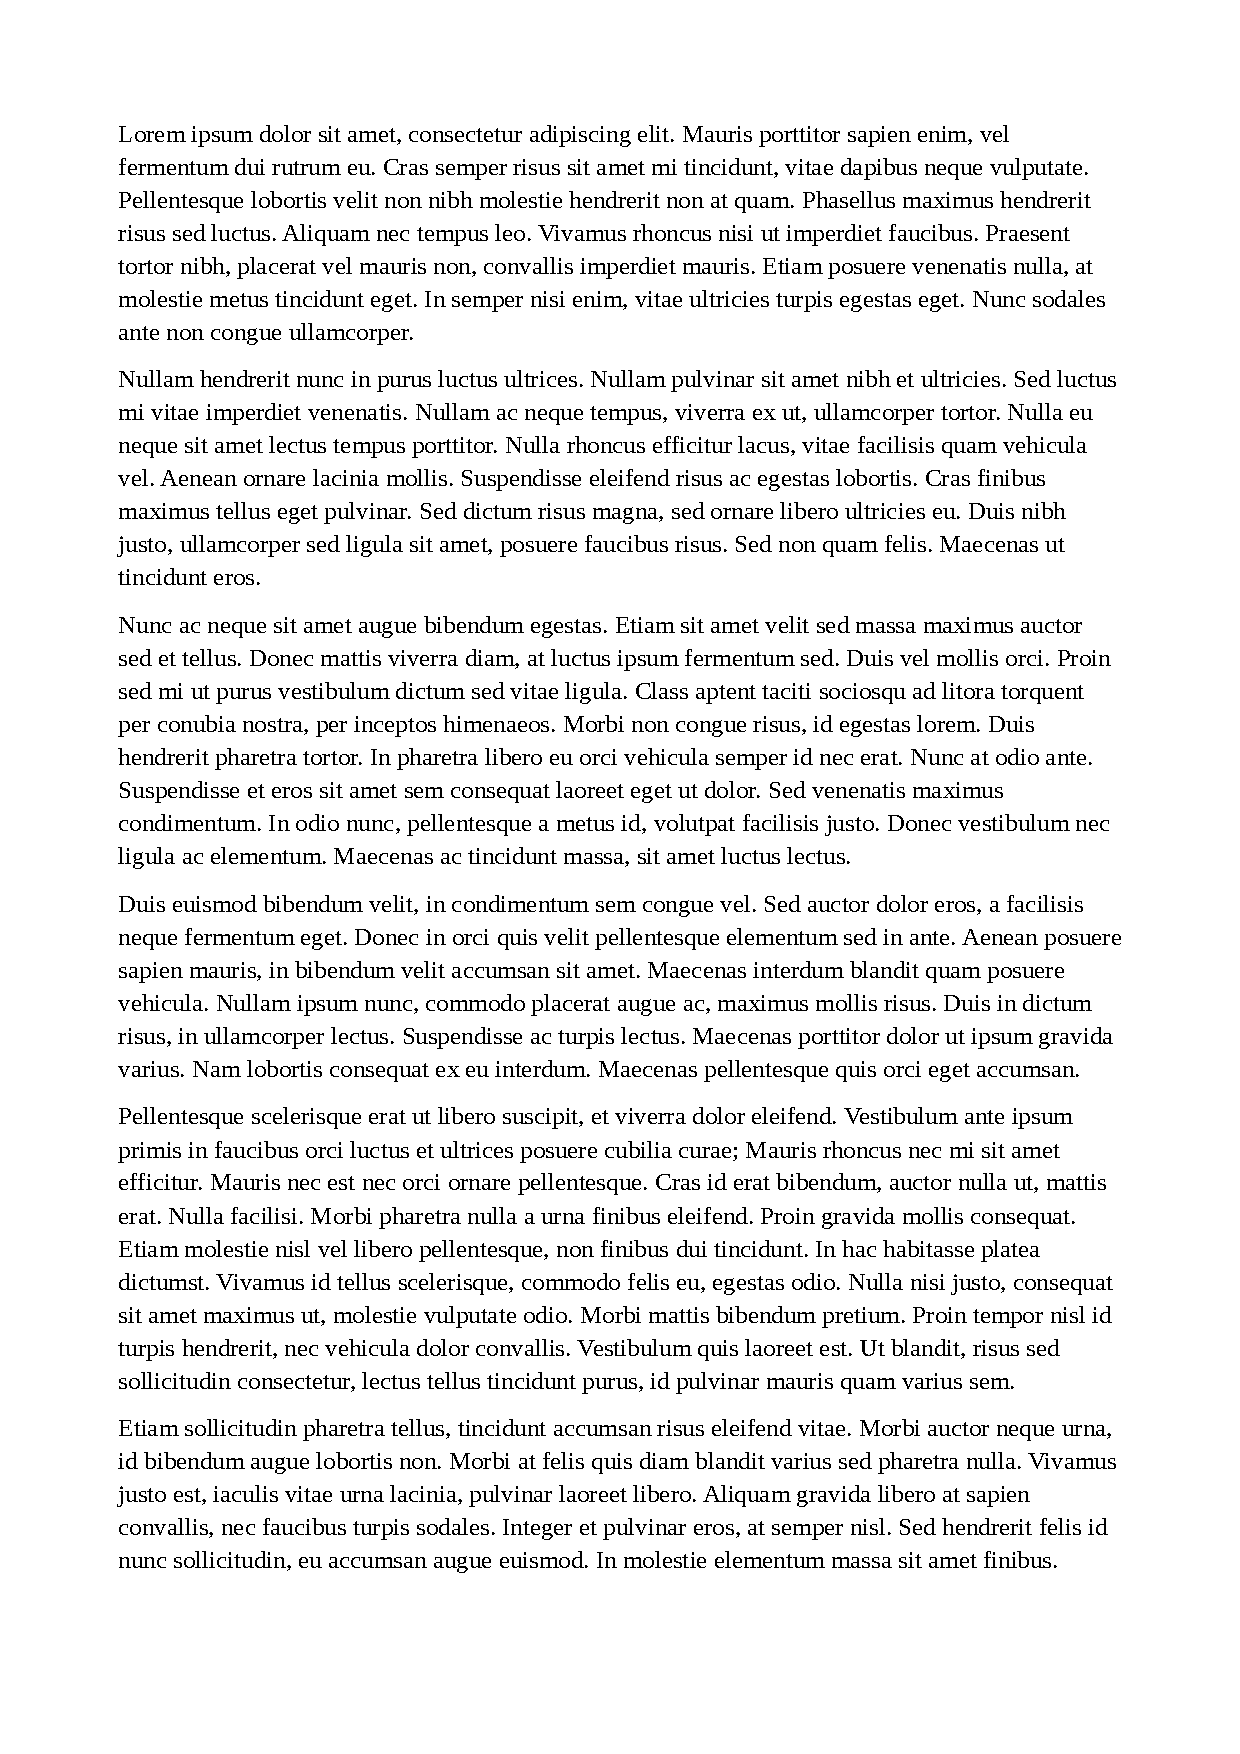
\includepdf[pages={1},scale=0.8,pagecommand=\chapter{Texto Texto Texto Texto}\label{apen:apendiceA}]{appendix/apendiceA}
\includepdf[pages={2-},scale=0.80,pagecommand={}]{appendix/apendiceA}

%%coloca o identificador do anexo/apendice somente na primeira página

\includepdf[pages={1},scale=0.80,pagecommand=\chapter{Texto Texto Texto}\label{apen:apendiceB}]{appendix/apendiceB}


%%coloca o identificador do anexo/apendice somente na primeira página
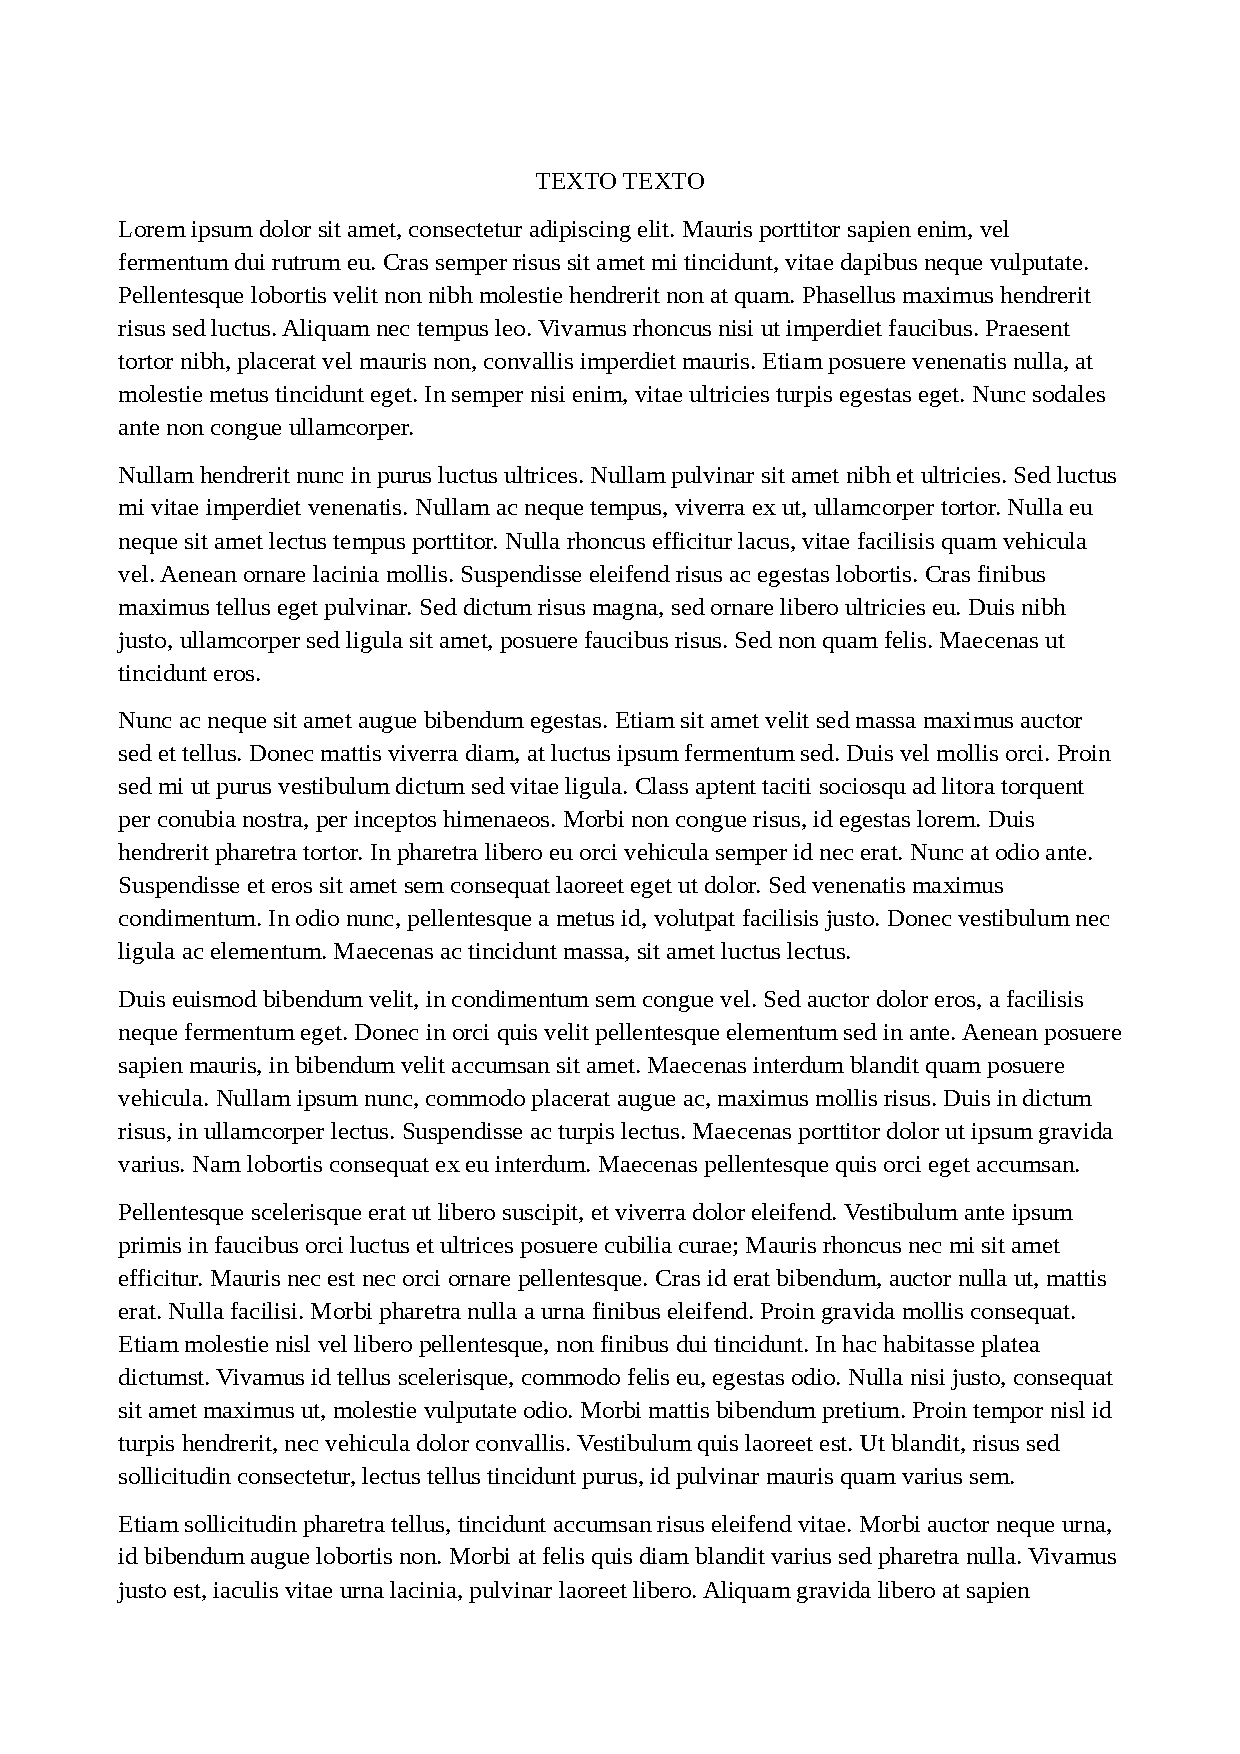
\includepdf[pages={1},scale=0.80,pagecommand=\chapter{Texto Texto}\label{apen:apendiceC}]{appendix/apendiceC}
\includepdf[pages={2},scale=0.80,pagecommand={}]{appendix/apendiceC}


\addtocontents{toc}{\endgroup}
\end{apendicesenv}




% ----------------------------------------------------------
% Anexos
% ----------------------------------------------------------

% ----------------------
% força para que não exiba subtítulos em apêndices no sumário
% -----------------------

\begin{anexosenv}
\addtocontents{toc}{\protect\setcounter{tocdepth}{1}}
\makeatletter
\addtocontents{toc}{%
  \begingroup
  \let\protect\l@chapter\protect\l@section
  \let\protect\l@section\protect\l@subsection
}
\makeatother
% Imprime uma página indicando o início dos apêndices
% \partapendices

%%coloca o identificador do anexo/apendice somente na primeira página
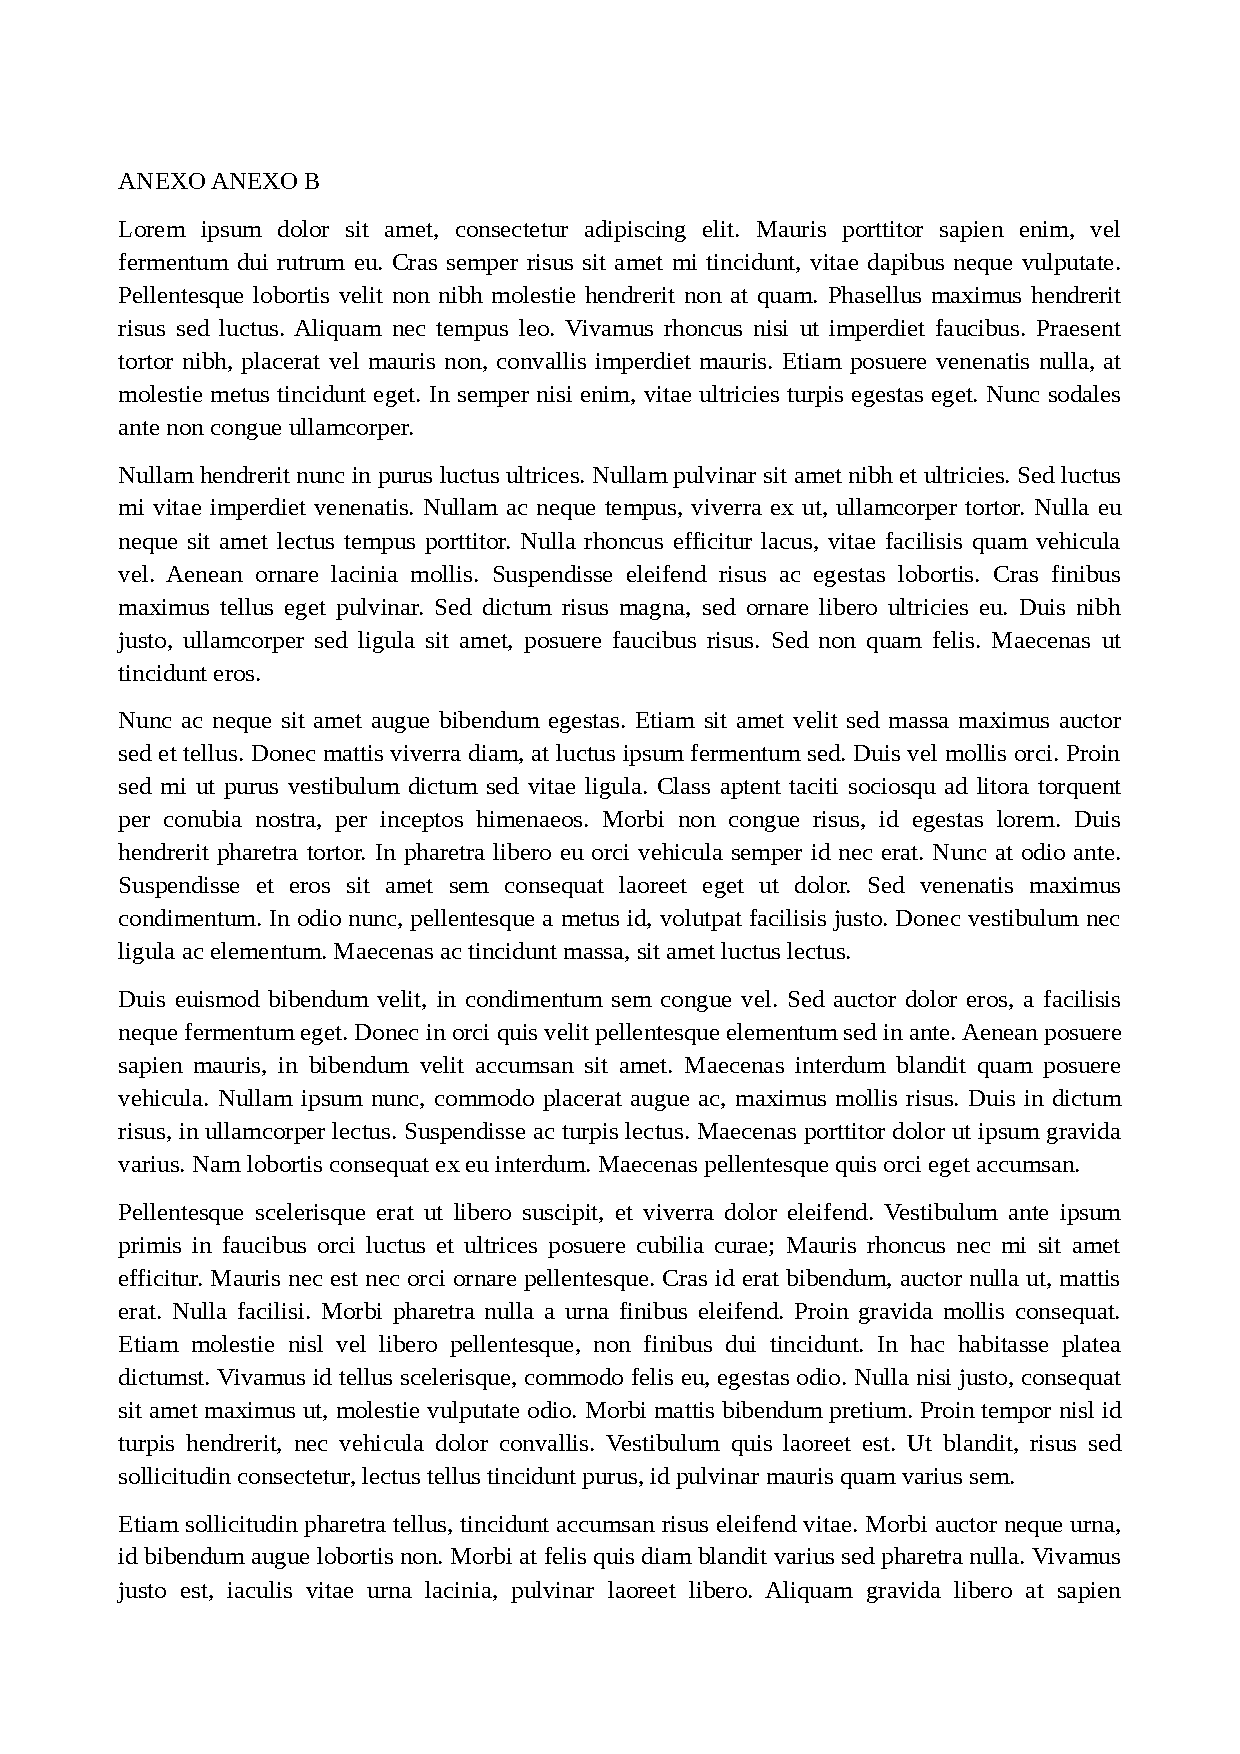
\includepdf[pages={1},scale=0.8,pagecommand=\chapter{Texto Texto Texto Texto}\label{anex:anexob}]{anexos/anexoB}
\includepdf[pages={2-},scale=0.80,pagecommand={}]{anexos/anexoB}

%%coloca o identificador do anexo/apendice somente na primeira página
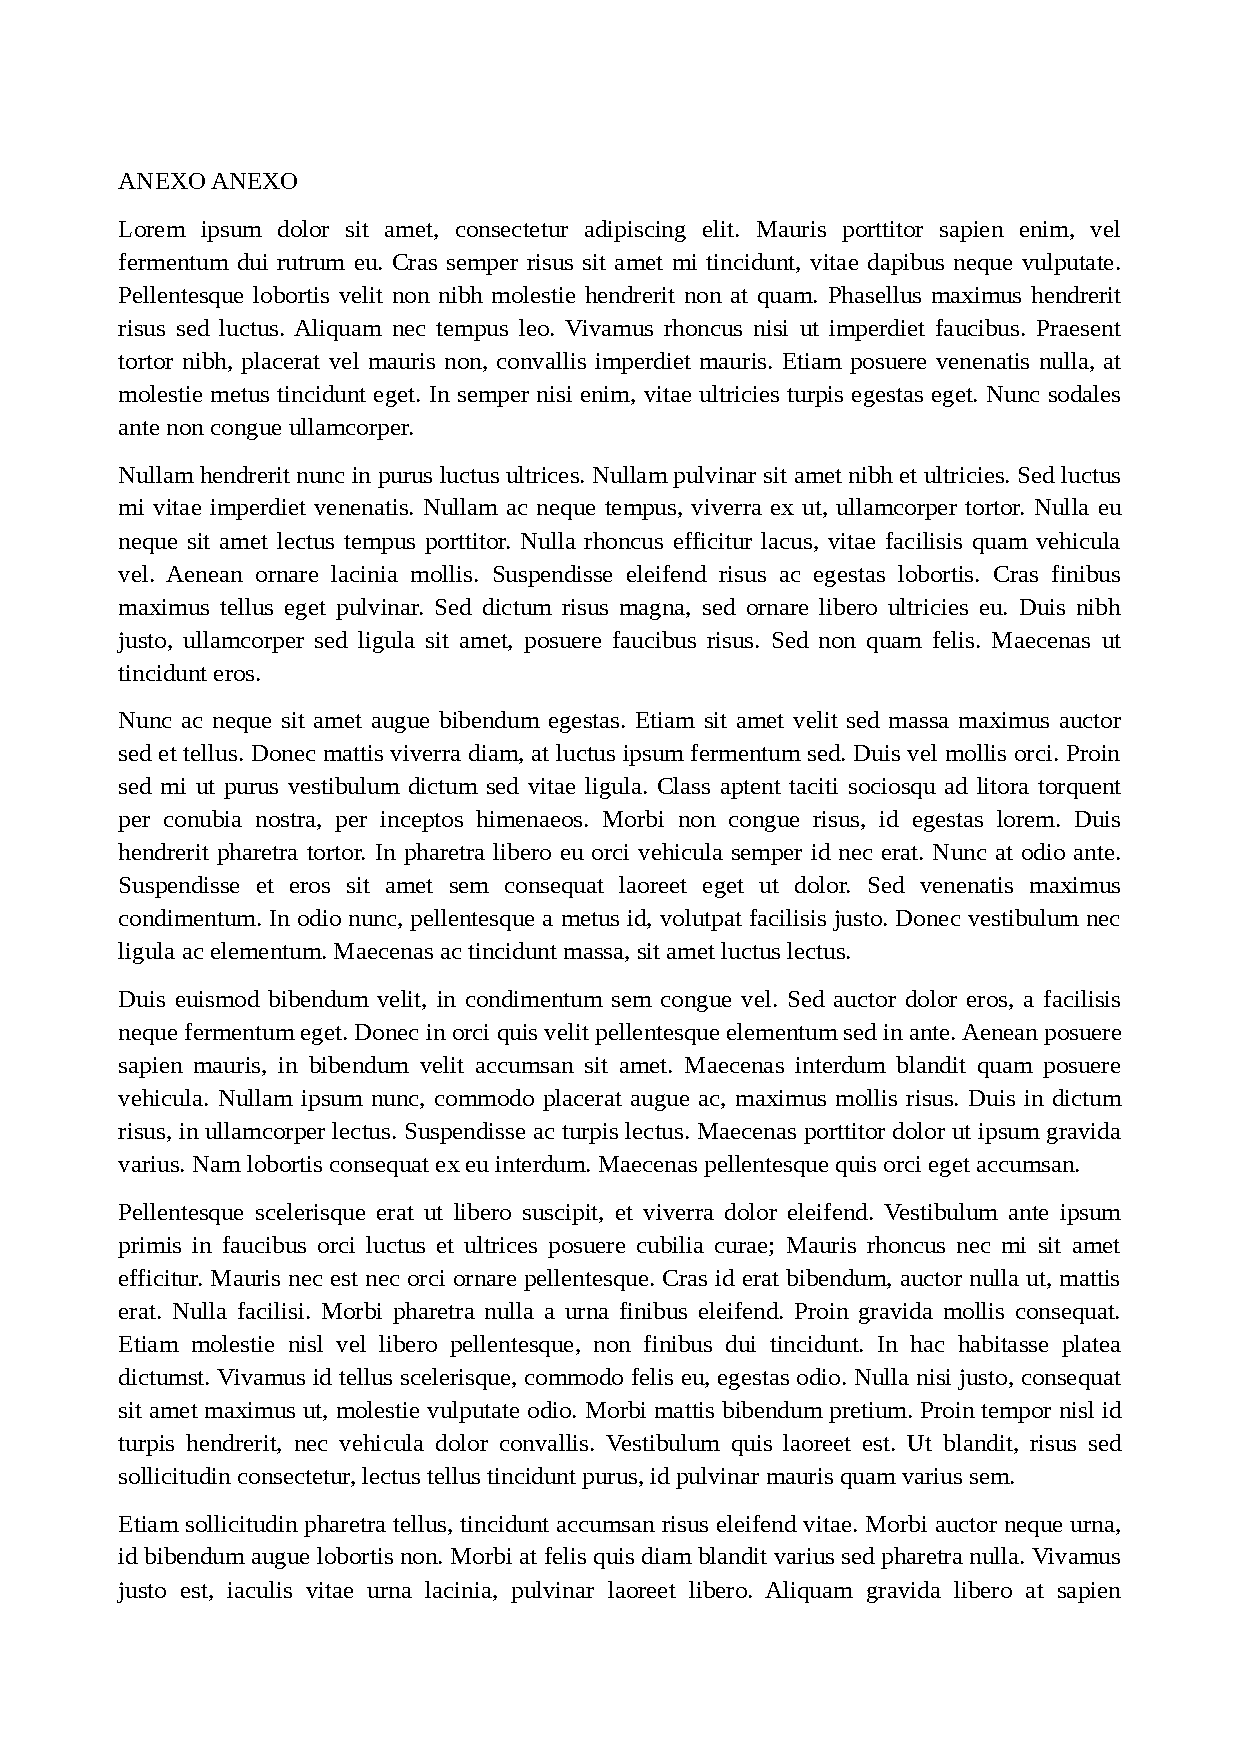
\includepdf[pages={1},scale=0.8,pagecommand=\chapter{Texto Texto Texto Texto}\label{anex:anexoa}]{anexos/anexoA}
\includepdf[pages={2-},scale=0.80,pagecommand={}]{anexos/anexoA}

\addtocontents{toc}{\endgroup}
\end{anexosenv}





\printindex


\end{document}
